\section{Validity Against Human Data}\label{sec:validity}
% Budget 2.0 pages with Fig 8.
\begin{figure}[t]
\centering
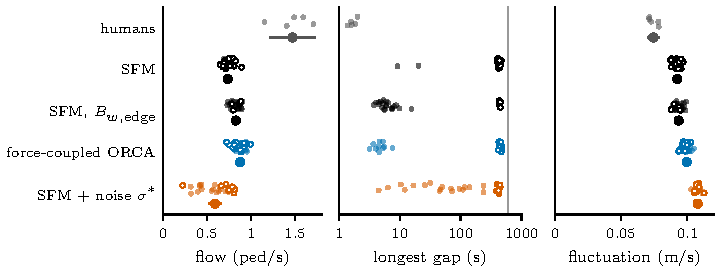
\includegraphics[width=\textwidth]{../figures/fig8_croma.pdf}
\caption{Flow through the entrance, longest time gap between successive passages (log scale) and waiting-zone velocity fluctuation for the five CroMa runs at $w=0.8$\,m and for each model variant in the matched geometry, with single runs as small points and means with 95\% intervals beside them. Humans are grey, C1 black (published mode open, corrected-forward filled, with jamb $B_w=0.04$ square), C3 RVO2 blue and C1 $+\,\sigma^\ast$ vermillion.}
\label{fig:croma}
\end{figure}
%
The deadlocks of Sects.~\ref{sec:physics} and~\ref{sec:attribution} are properties of the model. Whether real crowds show anything like them at the same width is a separate question, and we ask it like for like. The CroMa experiments~\cite{fzj_ped20219} include \EtenHumanN\ runs at an entrance width of 0.8\,m, two with a 2.0\,m corridor behind the entrance and three with a 0.21\,m one. We built their geometry: a walled holding area of $7.8\times8.6$\,m, the entrance, and corridor walls of the run's length, with the number of agents and the corridor length matched run by run (five model runs per human run and variant, 25 per variant). Three differences remain and are stated rather than fixed: model agents start at rest, their start positions lie farther from the entrance, and the barriers beyond the entrance are straight walls. Five variants were run for up to 600\,s: C1 in the published mode, where the jamb and corridor walls meeting at the door edge both act on an agent; C1 corrected-forward, where only the nearer of the two acts; C1 corrected-forward with the wall range at the jambs reduced to $B_w=0.04$\,m; C3 RVO2; and C1 $+\,\sigma^\ast$. Model and human trajectories went through the same estimator: passages through the entrance plane give the flow (first to last passage) and the time gaps between successive passages, and in the waiting zone, 0.3--2.5\,m in front of the entrance, the velocity fluctuation is the standard deviation of each agent's smoothed velocity (Savitzky--Golay, 1.48\,s) relative to the mean of its neighbours within 0.74\,m, at local mean speed below 0.3\,m/s. Means carry Student-$t$ 95\% intervals over runs.

\paragraph{Humans flow without deadlock.}
Every human run empties the holding area. The flow is \EtenHumanFlow\ [\EtenHumanFlowLo, \EtenHumanFlowHi]\,ped/s (runs \EtenHumanFlowMin--\EtenHumanFlowMax), \EtenLongHumanFlow\ with the long corridor and \EtenShortHumanFlow\ with the short one; the longest gap between passages averages \EtenHumanGap\,s and never exceeds \EtenHumanGapMax\,s, and a run has on average \EtenHumanGapsTwo\ gaps longer than 2\,s. The waiting-zone fluctuation is \EtenHumanFluct\ [\EtenHumanFluctLo, \EtenHumanFluctHi]\,m/s.

\paragraph{Every model variant deadlocks or flows at about half the human rate.}
No model variant reproduces this. C1 deadlocks in \EtenCPubDeadlock\ of 25 runs in the published mode and in \EtenCOneDeadlock\ in the corrected-forward mode (completion \EtenCPubComplete\ and \EtenCOneComplete, upper Wilson bound \EtenCPubCompleteHi, against \EtenHumanN\ of \EtenHumanN\ human runs). With the jamb wall range reduced to $B_w=0.04$\,m, \EtenCEdgeComplete\ runs complete and \EtenCEdgeDeadlock\ still deadlock. C3 RVO2 never deadlocks but completes only \EtenCThreeComplete\ runs within 600\,s, the other \EtenCThreeCapped\ still moving at the cap, and C1 $+\,\sigma^\ast$ completes \EtenCSigComplete. Whatever the variant, the flow, counted up to the deadlock where there is one, is \EtenCSigFlowRatio--\EtenCThreeFlowRatio\ of the human flow: \EtenCOneFlow\ [\EtenCOneFlowLo, \EtenCOneFlowHi]\,ped/s for corrected-forward C1 (ratio \EtenCOneFlowRatio\ [\EtenCOneFlowRatioLo, \EtenCOneFlowRatioHi]) and \EtenCThreeFlow\ [\EtenCThreeFlowLo, \EtenCThreeFlowHi]\,ped/s for C3 RVO2 (ratio \EtenCThreeFlowRatio\ [\EtenCThreeFlowRatioLo, \EtenCThreeFlowRatioHi]). Passages come in bursts separated by long gaps: \EtenCThreeGapsTwo--\EtenCOneGapsTwo\ gaps longer than 2\,s per run against \EtenHumanGapsTwo, and a mean longest gap of \EtenCThreeGap--\EtenCPubGap\,s for the deterministic variants and \EtenCSigGap\,s with noise, against \EtenHumanGap\,s (Fig.~\ref{fig:croma}). Noise turns deadlocks into long stalls and lowers the flow further. The model's waiting zone is also more agitated than the human one, \EtenCPubFluct--\EtenCSigFluct\,m/s against \EtenHumanFluct\,m/s. No agent leaves the walkable area in any run. The deficit does not depend on the corridor: with the long one humans reach \EtenLongHumanFlow\,ped/s and the model variants \EtenCSigLongFlow--\EtenCThreeLongFlow, with the short one \EtenShortHumanFlow\ and \EtenCSigShortFlow--\EtenCThreeShortFlow.

\paragraph{Wall treatment at door edges.}
Three points follow for practitioners who simulate narrow doors with a social force model. First, where a jamb and a corridor wall meet at a door edge, summing the force of the two segments counts the edge twice; the nearest point on the union of the walls counts it once and should be the default. Second, the range of the wall force at the door edges sets the stuck-alone margin of Eq.~\eqref{eq:stuck}. Before deadlock statistics at a narrow door are read as crowd behaviour, $g_{\max}(r)$ should be compared with $m v_0/\tau$ over the agent population, because a deadlock rate may measure only this margin. Third, removing deadlocks is not calibrating capacity: the reduced jamb range lets \EtenCEdgeComplete\ of 25 runs complete but leaves the flow at \EtenCEdgeFlowRatio\ of the human value, and matched noise, which reproduces ORCA's completion in the room, turns deadlocks into stalls with a mean longest gap of \EtenCSigGap\,s. A narrow-door model should be checked against the flow and gap statistics of matched experiments, not against completion alone.
